\section{Henkul\"are Homologie}
    Aus homologischer Sicht, ist die Henkelzerlegung sehr \"ahnlich zu der CW-Struktur eines zellul\"aren Komplexes, auch wenn die Ans\"atze nicht identisch sind. Die Konstruktion der Verklebung eines Henkels als Randsumme mit der Einheitskugel ist bei diesen \"Uberlegungen nachteilhaft, da dort keine kanonischen Inklusionen \(\mathcal{W},\mathbb{D}^n\hookrightarrow\mathcal{W}+\Psi^k\) existieren. Folglich sei \(\mathcal{W}+\Psi^k\) im Folgenden als Summe von \(\mathcal{W}\) mit \(\mathbb{D}^k\times\mathbb{D}^{n-k}\) verstanden. Dies ist m\"oglich da die beiden Ans\"atze hom\"oomorphe Mannigfaltigkeiten liefern. Folgende Konstruktion verl\"auft nahezu analog zu \cite{hatcher2002algebraic} [Section 2.2, Cellular Homology]. Der einzige Unterschied besteht darin, dass die Henkelzerlegung nicht von der leeren Menge ausgehend konstruiert wird, sodass statt der langen exakten Folge der Paare \(\left(\mathcal{W}_k,\mathcal{W}_{k-1}\right)\) eine lange exakte Folge von Tripeln \(\left(\mathcal{W}_k,\mathcal{W}_{k-1},\mathcal{M}\times\mathbb{I}\right)\) betrachtet werden muss. Es gelten folgende Eigenschaften (Vergleiche Hatcher Section 2.2 Lemma 2.34)
    \begin{lemma}\label{lem:handular_homology}
        Ist \(\mathcal{W}\) ein Kobordismus mit Henkelzerlegung \(\mathcal{W}_k\), so gilt:
        \begin{enumerate}
            \item[i)] \(H_k\left(\mathcal{W}_m,\mathcal{W}_{m-1}\right)\not=0\) genau dann, wenn \(m=k\) ist. Dann ist diese frei abelsch und von den Kernen der \(k\)-Henkel erzeugt.
            \item[ii)] Die Abbildung \(H_k\left(\mathcal{W}_m,\mathcal{M}\right)\to H_k\left(\mathcal{W},\mathcal{M}\right)\) ist ein Isomorphismus f\"ur \(k<m\) und ein Epimorphismus f\"ur \(k=m\).
            \item[iii)] \(H_k\left(\mathcal{W}_m,\mathcal{M}\right)=0\) f\"ur \(k>m\).
        \end{enumerate}
    \end{lemma}
    \begin{proof}
        \subsubsection{i)}
            Die Projektion \(\left(\mathbb{D}^m\times\mathbb{D}^{n-m},\mathbb{S}^{m-1}\times\mathbb{D}^{n-m}\right)\to\left(\mathbb{D}^m,\mathbb{S}^{m-1}\right)\) ist eine Homotpie\"aquivalenz, und bildet einen Henkel auf seinen Kern ab. Da ein Henkel in \(\mathcal{W}_m\) stets an \(\mathcal{W}_{m-1}\) angebracht ist, gilt
            \begin{align*}
                H_k\left(\mathcal{W}_m,\mathcal{W}_{m-1}\right)&\cong\Tilde{H}_k\bigg(\bigvee_{j=1}^{c_m}\mathbb{D}^m\times\mathbb{D}^{n-m}\mathrel{/}\mathbb{S}^{m-1}\times\mathbb{D}^{n-m}\bigg)\\[-6pt]
                &\cong\bigoplus_{j=1}^{c_m}\Tilde{H}_k\left(\mathbb{D}^m\mathrel{/}\mathbb{S}^{m-1}\right)\cong\bigoplus_{j=1}^{c_m}\Tilde{H}_k\left(\mathbb{S}^m\right)\,.
            \end{align*}
            Demnach ist \(H_k\left(\mathcal{W}_k,\mathcal{W}_{k-1}\right)\) f\"ur \(m\not=k\) trivial und sonst zu \(\mathbb{Z}^{c_k}\) isomorph. Die Generatoren der \(\mathbb{Z}\)-Anteile stehen hierbei in bijektiver Korrespondenz zu den Kernen der Henkel, also auch zu den Henkeln selbst.
            
        \subsubsection{ii) \& iii)}
            Die lange exakte Folge des Tripels \(\left(\mathcal{W}_m,\mathcal{W}_{m-1},\mathcal{M}\right)\) ist gerade
            \begin{center}
                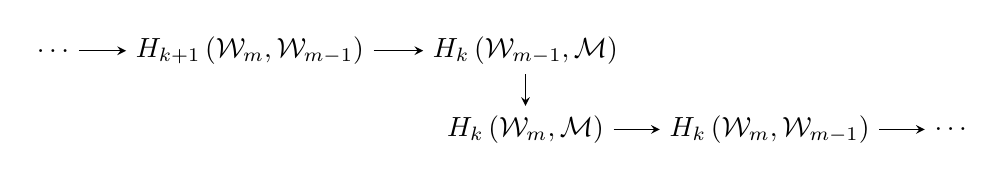
\begin{tikzpicture}
                    \path   node (A) at (-6, 1) {\(\dots\)}
                            node (B) at (-3.5, 1) {\(H_{k+1}\left(\mathcal{W}_m,\mathcal{W}_{m-1}\right)\)}
                            node (C) at (0, 1) {\(H_k\left(\mathcal{W}_{m-1},\mathcal{M}\right)\)}
                            node (D) at (0, 0) {\(H_k\left(\mathcal{W}_m,\mathcal{M}\right)\)}
                            node (E) at (3.1, 0) {\(H_k\left(\mathcal{W}_m,\mathcal{W}_{m-1}\right)\)}
                            node (F) at (5.4, 0) {\(\dots\)};
                    \draw[-stealth] (A.east) -- (B.west);
                    \draw[-stealth] (B.east) -- (C.west);
                    \draw[-stealth] (C.south) -- (D.north);
                    \draw[-stealth] (D.east) -- (E.west);
                    \draw[-stealth] (E.east) -- (F.west);
                \end{tikzpicture}
            \end{center}
            F\"ur \(m\not=k\) oder \(m\not=k-1\) ist entweder die erste oder letzte Gruppe trivial und die mittlere Abbildung damit ein Epimorphismus oder ein Monomorphismus. Dies zeigt ii). Mit \(H_k\left(\mathcal{W}_{-1},\mathcal{M}\right)=0\) ergibt dies iii).
    \end{proof} 
    Durch dem aus der langen exakten Folge stammenden Differential
    \begin{equation}\label{eq:differential}
        \partial_k\colon H_k\left(\mathcal{W}_k,\mathcal{W}_{k-1}\right)\to H_{k-1}\left(\mathcal{W}_{k-1},\mathcal{M}\right)
    \end{equation}
    und der von der Quotientenabbildung induzierten Abbildung 
    \[q_k^*\colon H_{k-1}\left(\mathcal{W}_{k-1},\mathcal{M}\right)\to H_{k-1}\left(\mathcal{W}_{k-1},\mathcal{W}_{k-2}\right)\]
    kann nun ein weiteres Differential durch \(\dx_k:=q_k^*\circ\partial_k\) definiert werden, welches im Folgenden genauer untersucht werde. Die Homologiegruppen \(H_k\left(\mathcal{W}_k,\mathcal{W}_{k-1}\right)\) mit diesem Differential als Zellkomplex ergeben neue Homologiegruppen \(H_k^{Hen}\left(\mathcal{W}\right)\). F\"ur diese gilt analog zu Hatcher Satz 2.35
    \[H_*^{Hen}\left(\mathcal{W}\right)\cong H_*\left(\mathcal{W},\mathcal{M}\right)\,,\]
    was jedoch im Folgenden nicht weiter ben\"otigt werde. 
    \begin{remark}\label{rem:incl_epi}
        Sei \(\left(\mathcal{W}^n,\mathcal{M},-\right)\) ein H-Kobordismus. Dann gilt wegen \(\mathcal{M}\simeq\mathcal{W}\) auch
        \[H_0\left(\mathcal{W}_1,\mathcal{M}\right)\cong H_0\left(\mathcal{W},\mathcal{M}\right)\cong0\,.\]
        Die lange exakte Folge des Paares \(\left(\mathcal{W}_1,\mathcal{M}\right)\) ist dann
        \[\dots\to H_1\left(\mathcal{W}_1,\mathcal{M}\right)\to H_0\left(\mathcal{M}\right)\mathop{\hookrightarrow}^{\iota^*}H_0\left(\mathcal{W}_1\right)\to0\to\dots\,,\]
        sodass \(\iota^*\) ein Epimorphismus ist. Folglich kann \(\mathcal{W}_1\) nicht mehr Zusammenhangskomponenten als \(\mathcal{M}\) besitzen.
    \end{remark}
    Existieren keine \(j\)-Henkel f\"ur \(j<k\), ist \(\mathcal{W}_{k-1}\cong\mathcal{M}\times\mathbb{I}\), und die Abbildung \(q_{k+1}^*\) ist gleich der Identit\"at, sodass \(\dx_{k+1}=\partial_{k+1}\) gilt. In diesem Fall existiert eine intuitive Beschreibung durch Schnittzahlen. 
    
    \subsection{Schnittzahlen und der Whitney-Trick}
        Seien \(\mathcal{M}^k\) und \(\mathcal{N}^{n-k}\) transversale Untermannigfaltigkeiten von \(\mathcal{W}^n\), wobei \(\mathcal{N}\) und das Normalenb\"undel von \(\mathcal{M}\) orientiert seien. Sei weiter \(\mathcal{M}\subset U\subseteq\mathcal{W}\) eine Tubenumgebung, sodass in allen Punkten \(p\in\mathcal{M}\cap\mathcal{N}\) die Faser \(U_p\) eine Umgebung von \(p\) in \(\mathcal{N}\) sei (aufgrund der Transversalit\"at kann dies stets gew\"ahrleistet werden). Dann ergeben sich induzierte lokale Orientierungen
        \[H_n\left(N\mathcal{M}\right)\cong H_n\left(U\right)\to H_n\left(U,U\setminus\mathcal{M}\right)\cong H_{n-k}\left(U_p,U_p\setminus 0\right)\]
        und
        \[H_{n-k}\left(\mathcal{N}\right)\cong H_{n-k}\left(\mathcal{N},\mathcal{N}\setminus p\right)\,.\]
        Da die Inklusion \(U_p\to\mathcal{N}\) Isomorphismen
        \[H_{n-k}\left(U_p,U_p\setminus p\right)\cong H_{n-k}\left(\mathcal{N},\mathcal{N}\setminus p\right)\]
        induziert, k\"onnen diese lokalen Orientierungen verglichen werden. In einem Punkt \(p\) sei nun \(\epsilon_p=1\), falls diese Orientierungen \"ubereinstimmen, und \(-1\) sonst. Die Schnittzahl sei
        \[\left[\mathcal{M},\mathcal{N}\right]:=\mathop{\sum\epsilon_p}_{p\hspace{1pt}\in\mathcal{M}\hspace{1pt}\cap\hspace{1pt}\mathcal{N}}\,.\]
        Seien nun alle Kerne von Henkeln \(\Psi^k,\Psi^{k+1}\) beliebig orientiert. Dies induziert sowohl eine Orientierung des Normalenb\"undels von \(\Sigma^k\), als auch eine Orientierung der Anklebesph\"are \(\Lambda^{k+1}\). Folglich k\"onnen im Falle eines transversalen Schnittes die Schnittzahlen \(\left[\Sigma^k,\Lambda^{k+1}\right]\) betrachtet werden, und es gilt (!)
        \[\dx\Psi^{k+1}=\sum_{j=1}^{c_k}\left[\Sigma_j^k,\Lambda^{k+1}\right]\Psi_j^k\,.\]
        
        \begin{proposition}[Whitneys Trick]
            Seien \(\mathcal{M}^m\) und \(\mathcal{N}^n\) zusammenh\"angende Untermannigfaltigkeiten der einfach zusammenh\"angenden Mannigfaltigkeit \(\mathcal{V}^{n+m}\), wobei \(n+m\geq5\), \(n\geq2\) und \(m\geq3\) gelte. Sei \(\mathcal{M}\) und das Normalenb\"undel von \(\mathcal{N}\) orientiert. Seien \(p,q\in\mathcal{M}\cap\mathcal{N}\) derart, dass \(\epsilon_p+\epsilon_q=0\) gelte, so existiert eine Isotopie \(h\colon\mathcal{M}\times\mathbb{I}\to\mathcal{V}\) die in einer Umgebung von \(\mathcal{M}\cap\mathcal{N}\setminus\{p,q\}\) station\"ar ist, und \(h_1\left(\mathcal{M}\right)\cap\mathcal{N}=\mathcal{M}\cap\mathcal{N}\setminus\{p,q\}\) gilt.
        \end{proposition}
        \begin{proof}
            Siehe \cite{milnor1965hcobordism} Seite 71 Satz 6.6.
            \renewcommand\qedsymbol{\(\cancel{qed}\)}
        \end{proof}
        Die Forderung der hohen Dimensionalit\"at ergibt sich daraus, dass eine \(2\)-dimensionale Scheibe in \(\mathcal{M}^n\) eingebettet werden muss, wof\"ur der schwache Einbettungssatz von Whitney ben\"otigt wird. Folglich muss \(n\geq 2\cdot2+1=5\) gelten. 
        
\section{Homologie- und Modifikationslemmata}
    Folgendes Lemma erkl\"art die simple Beziehung zwischen sich aufhebenden Henkeln und ist der Grund f\"ur die Forderung, dass der Kobordismus mindestens \(6\)-dimensional ist. Es ist eine (fast) direkte Folgerung aus dem Whitney-Trick.
    \begin{theorem}[Homologie-Lemma]\label{thm:homology}
        Besitzt eine Henkelzerlegung mit \(\mathcal{W}_{k-1}\cong\mathcal{M}\times\mathbb{I}\) eines mindestens \(6\)-di\-men\-sio\-na\-len Kobordismus \(\mathcal{W}\) keine \((j<k)\)-Henkel und gilt \(\dx\Psi^{k+1}=\Psi_i^k\), ist \(\Psi^{k+1}\) rechtsinvers zu \(\Psi_i^k\).
    \end{theorem}
    \begin{proof}
        Der Kern eines Henkels wird unter dem Differential auf seinen Rand, also auf die Anklebesph\"are abgebildet, die nach einer Isotopie als transversal zu allen G\"urteln von \(k\)-Henkeln angenommen werden kann. Aus Dimensiongr\"unden, sind dies lediglich endlich viele Punkte. Wegen
        \[\dx\Psi^{k+1}=\sum_{j=1}^{c_k}\Big[\Lambda^{k+1},\Sigma_j^k\Big]\Psi_j^k=\Psi_i^k\,,\]
        muss f\"ur \(j\not=i\) auch
        \[\Big[\Lambda^{k+1},\Sigma_j^k\Big]\mathop{=\sum\epsilon_p=}_{p\in\Sigma_j^k\cap\Lambda^{k+1}}0\]
        gelten, sodass stets Paare \(p,q\in\Lambda^{k+1}\cap\Sigma_j^k\) mit \(\epsilon_p+\epsilon_q=0\) existieren, die sich durch eine Isotopie gem\"a\ss{} dem Whitney-Trick aufheben. F\"ur \(i=j\) folgt analog, dass sich alle bis auf einen Punkt \(p\) mit \(\epsilon_p=1\) paarweise aufheben. Da sich \(\Psi^{k+1}\) und \(\Psi_i^{k+1}\) nun transversal und nur in \(p\) schneiden l\"asst sich der K\"urzungssatz anwenden.
    \end{proof}
    
    \begin{proposition}[Modifikationslemma]\label{prop:modification}
        F\"ur Henkel \(\Psi_1^k\) und \(\Psi_2^k\) existiert ein in \(\partial_+\mathcal{W}_k\) isotoper Henkel \(\Phi^k\simeq\Psi_1^k\) mit
        \[\dx\Phi^k=\dx\Psi_1^k+\dx\Psi_2^k\,.\]
    \end{proposition}
    \begin{proof}
        Dies folgt aus \cite{kosinski2013differential} Kapitel VIII Lemma 1.2.
    \end{proof}
